\section{Architecture du Système}

\subsection{Vue d'Ensemble de l'Architecture}

Running App adopte une architecture moderne en 3 tiers, séparant clairement la présentation, la logique métier et la persistance des données.

\begin{figure}[H]
\centering
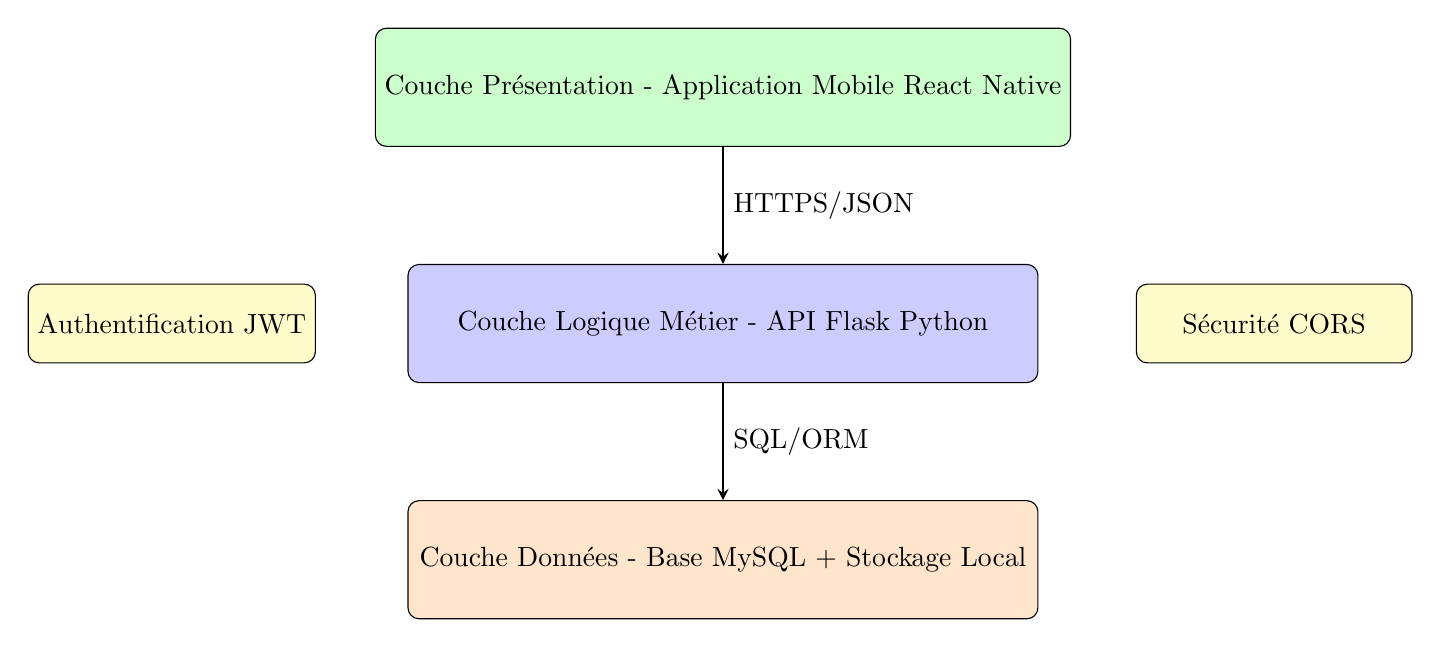
\begin{tikzpicture}[node distance=3cm]
    % Styles
    \tikzstyle{layer} = [rectangle, rounded corners, minimum width=8cm, minimum height=1.5cm, text centered, draw=black, fill=blue!10]
    \tikzstyle{component} = [rectangle, rounded corners, minimum width=3.5cm, minimum height=1cm, text centered, draw=black]
    \tikzstyle{arrow} = [thick,->,>=stealth]
    
    % Couches
    \node (mobile) [layer, fill=green!20] {Couche Présentation - Application Mobile React Native};
    \node (api) [layer, below of=mobile, fill=blue!20] {Couche Logique Métier - API Flask Python};
    \node (data) [layer, below of=api, fill=orange!20] {Couche Données - Base MySQL + Stockage Local};
    
    % Flèches
    \draw [arrow] (mobile) -- node[anchor=west] {HTTPS/JSON} (api);
    \draw [arrow] (api) -- node[anchor=west] {SQL/ORM} (data);
    
    % Composants détaillés
    \node (auth) [component, left of=api, xshift=-4cm, fill=yellow!20] {Authentification JWT};
    \node (cors) [component, right of=api, xshift=4cm, fill=yellow!20] {Sécurité CORS};
    
\end{tikzpicture}
\caption{Architecture 3-Tiers de Running App}
\end{figure}

\subsection{Composants Principaux}

\subsubsection{Frontend Mobile - React Native}

\begin{description}
    \item[\textbf{Navigation}] React Navigation v6 avec navigation par onglets
    \item[\textbf{État Global}] Context API pour la gestion d'état (Auth, Runs)
    \item[\textbf{Géolocalisation}] Expo Location pour le tracking GPS
    \item[\textbf{Cartographie}] React Native Maps avec Google Maps
    \item[\textbf{Stockage}] AsyncStorage pour la persistence locale
    \item[\textbf{Réseau}] Axios pour les appels API avec intercepteurs
\end{description}

\subsubsection{Backend API - Python Flask}

\begin{description}
    \item[\textbf{Framework}] Flask 2.3+ avec architecture modulaire par blueprints
    \item[\textbf{ORM}] SQLAlchemy pour la gestion des données
    \item[\textbf{Migrations}] Flask-Migrate pour l'évolution du schéma
    \item[\textbf{Authentification}] Flask-JWT-Extended pour les tokens JWT
    \item[\textbf{CORS}] Flask-CORS pour les requêtes cross-origin
    \item[\textbf{Validation}] Validation automatique des données JSON
\end{description}

\subsubsection{Base de Données - MySQL}

\begin{description}
    \item[\textbf{SGBD}] MySQL 8.0+ avec support des données JSON
    \item[\textbf{Structure}] Base normalisée avec relations optimisées
    \item[\textbf{Index}] Index sur les clés étrangères et champs de recherche
    \item[\textbf{Contraintes}] Contraintes d'intégrité référentielle
\end{description}

\subsection{Patterns Architecturaux Utilisés}

\subsubsection{MVC (Model-View-Controller)}

\begin{itemize}
    \item \textbf{Model :} Classes SQLAlchemy (User, Run, Stats)
    \item \textbf{View :} Composants React Native + réponses JSON API
    \item \textbf{Controller :} Routes Flask + logique métier dans services
\end{itemize}

\subsubsection{Repository Pattern}

\begin{itemize}
    \item Séparation entre logique métier et accès aux données
    \item Services dédiés pour chaque entité métier
    \item Réutilisabilité et testabilité améliorées
\end{itemize}

\subsubsection{API RESTful}

\begin{itemize}
    \item Respect des conventions REST (GET, POST, PUT, DELETE)
    \item Codes de statut HTTP appropriés
    \item Structure JSON standardisée pour les réponses
    \item Versioning de l'API prévu (/api/v1/)
\end{itemize}

\subsection{Flux de Données}

\subsubsection{Authentification}

\begin{enumerate}
    \item L'utilisateur saisit ses identifiants
    \item L'app mobile envoie les données à \texttt{POST /api/auth/login}
    \item L'API valide et retourne un token JWT
    \item Le token est stocké localement et inclus dans les requêtes suivantes
    \item Refresh automatique du token avant expiration
\end{enumerate}

\subsubsection{Enregistrement d'une Course}

\begin{enumerate}
    \item Démarrage du GPS et collecte des coordonnées
    \item Calculs en temps réel (distance, vitesse, durée)
    \item Sauvegarde locale pendant la course
    \item Envoi des données à \texttt{POST /api/runs} à la fin
    \item Synchronisation bidirectionnelle avec le serveur
\end{enumerate}

\subsection{Considérations de Performance}

\begin{itemize}
    \item \textbf{Optimisation GPS :} Mise à jour adaptative selon la vitesse
    \item \textbf{Cache local :} Données critiques stockées offline
    \item \textbf{Pagination :} Chargement par pages pour les listes
    \item \textbf{Compression :} Gzip activé sur l'API
    \item \textbf{Index DB :} Optimisation des requêtes fréquentes
\end{itemize}

\subsection{Gestion d'Erreurs}

\begin{description}
    \item[\textbf{Frontend}] Try-catch avec fallback gracieux et messages utilisateur
    \item[\textbf{Backend}] Middleware global de gestion d'erreurs avec logging
    \item[\textbf{Réseau}] Retry automatique et mode offline
    \item[\textbf{Validation}] Validation côté client et serveur
\end{description}